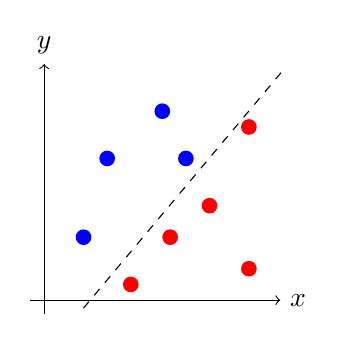
\begin{tikzpicture}[
  triangle/.style = {fill=blue!20, regular polygon, regular polygon sides=3 },
  ]
  \draw[->] (-5pt,0) -- (3,0) node[right] {$x$}; % x-axes
  \draw[->] (0,-5pt) -- (0,3) node [above] {$y$}; % y-axes

  \draw[dashed] (0.5,-0.1) -- ++(50:4.0);

  \node[fill,circle,inner sep=2,blue] at (0.5,0.8) {};
  \node[fill,circle,inner sep=2,blue] at (0.8,1.8) {};
  \node[fill,circle,inner sep=2,blue] at (1.8,1.8) {};
  \node[fill,circle,inner sep=2,blue] at (1.5,2.4) {};

  \node[fill,circle,inner sep=2,red] at (1.1,0.2) {};
  \node[fill,circle,inner sep=2,red] at (2.6,0.4) {};
  \node[fill,circle,inner sep=2,red] at (1.6,0.8) {};
  \node[fill,circle,inner sep=2,red] at (2.6,2.2) {};
  \node[fill,circle,inner sep=2,red] at (2.1,1.2) {};

\end{tikzpicture}


%%% Local Variables:
%%% mode: latex
%%% TeX-master: "../figs"
%%% End:
